\section{Programming with \name}
\label{sec:motivation}

\subsection{RDT Definition}

\begin{figure}
\begin{codehaskell}
data Ctr = Inc

type Counter = [Ctr]

read :: Counter -> () -> (Int, Maybe Ctr)
read hist _ = (length hist, Nothing)

inc :: Counter -> () -> ((), Maybe Ctr)
inc hist _ = ((), Just Inc)
\end{codehaskell}
%\captionsetup{singlelinecheck=off}
\caption{Definition of a counter expressed in Quelea.}
\label{fig:ex}
\end{figure}

Figure~\ref{fig:ex} shows the implementation of a counter RDT in
\name. The data type \cf{Ctr} represents the counter's effect type.
Every RDT in \name is associated with an effect type that specifies
the effects allowed on the objects of that type.  An RDT is defined
merely a list of its effects. The type of an RDT operation is an
instance of the following type, written in Haskell syntax:

\begin{codehaskell}
type Operation e a r = [e] -> a -> (r, Maybe e)
\end{codehaskell}

\noindent An operation on an RDT accepts a list of effects (the
\emph{history} of updates representing the state of the object at some
replica), and an input argument, and returns a result along with an
optional effect.  While a read-only operation (eg., \rcf{read})
generates no effect (i.e., it returns \cf{Nothing}), a write-only
operation (eg., \rcf{inc}) returns a new effect.

\subsection{Anomalies under Eventual Consistency}

\begin{figure}[ht]
\centering
\subfigure[Monotonicity Violation]{\label{fig:monotonicityViolation}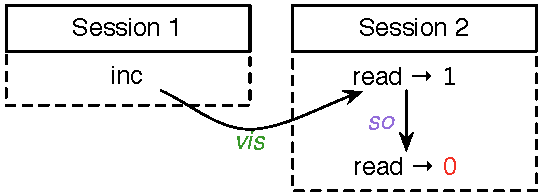
\includegraphics[width=0.55\columnwidth]{Figures/monotonicityViolation}}
%\hfill
\hspace*{0.5in}
\subfigure[Missing
Update]{\label{fig:missingUpdate}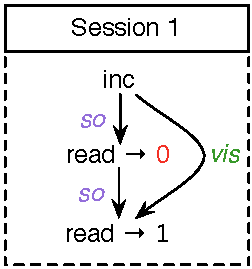
\includegraphics[scale=0.9]{Figures/missingUpdate}}
\hfill
\caption{Anomalies possible under eventual consistency for the counter
read operation.}
\label{fig:counter_anomalies}
\end{figure}

Observe that the counter RDT does not admit a decrement operation.
Therefore, the value of a counter should appear to be monotonically
increasing. Indeed, this property is what makes the RDT useful to
implement, for example, a video view counter on Youtube.
Unfortunately, the monotonicity invariant can be violated in an
eventually consistent execution.

Consider the execution shown in
Figure~\ref{fig:monotonicityViolation}. Session 1 performs an
\rcf{inc} operation on the counter, while Session 2 performs two
\rcf{read} operations. The first \rcf{read} witnesses the effect of
\rcf{inc} from Session 1, hence returns 1. The second \rcf{read},
however, does not witness \rcf{inc}, possibly because it was served by
a replica that has not yet merged the \rcf{inc} effect. It returns 0,
thus violating the monotonicity invariant. 

In order for counter's value to appear monotonically increasing, the
second \rcf{read} should also witness the effect of \rcf{inc}, because
it was witnessed by the preceding \rcf{read}. Because eventually
consistent \rcf{read} operations do not ensure this property,
\rcf{read} operations need to be executed at a stronger consistency
level. The choice of consistency level must guarantee that if
a \rcf{read} witnesses an \rcf{inc} effect, all the subsequent
\rcf{read} operations on the same counter object also witness that
effect. If we let $\sameobjZ$ relate effects over the same
object, we can formalize this requirement using visibility ($\visZ$)
and session order ($\soZ$) relations:
\begin{cmathpar}
\begin{array}{l}
\forall (a : \rcf{inc}), (b,c : \rcf{read}).
\; \vis{a}{b} \conj \so{b}{c} \conj \sameobj{b}{c} \Rightarrow \vis{a}{c} 
\end{array}
\end{cmathpar}
The above formula is in fact a valid specification that can be
associated with counter RDT operations in \name. Note that the
specification captures the guarantees required to enforce the
monotonicity invariant with respect to the abstract model of the store
described in \S~\ref{sec:sysmod}. In particular, the specification
does not refer to the low-level details of any specific data store.
Our observation is that if consistency levels can also be specified in
a similar manner, we can eliminate the need for the application
programmer to understand the low-level nuances of the data store to
enforce the required invariants; understanding their semantics in the
abstract model is enough. In the following sections, we demonstrate
that this is indeed possible. We first introduce our specification
language.

\subsection{Specification Language}

\begin{figure}
\begin{smathpar}
\renewcommand{\arraystretch}{1.2}
\begin{array}{rclcl}
\multicolumn{5}{c}{
  {a,b} \in \mathtt{EffVar} \qquad \qquad
  {\sf Op} \in \mathtt{OperName}
}\\
\cv 		& \in & \mathtt{Spec} 	& \coloneqq & \forall (a : \tau).\cv
        \ALT \forall a.\cv \ALT \pi \\
\tau		& \in	& \mathtt{EffType}	& \coloneqq &  {\sf Op}
        \ALT \tau \vee \tau \\
\pi			&	\in & \mathtt{Prop} & \coloneqq & \true \ALT R(a,b)
        \ALT \pi \vee \pi \\
			  & 		&	 &  \ALT & \pi \wedge \pi \ALT \pi \Rightarrow \pi \\
R				& \in & \mathtt{Relation}	& \coloneqq & \visZ \ALT \soZ
        \ALT \sameobjZ \ALT = \\
				&			&	 &  \ALT & R \cup R \ALT R \cap R \ALT R^+ \\
\end{array}
\end{smathpar}
\caption{Contract language.}
\label{fig:specification-lang}
\end{figure}

The syntax of our specification language is shown in Figure
~\ref{fig:specification-lang}. The language is based on first-order logic
(FOL), and admits prenex universal quantification over typed and
untyped effect variables. We use a special effect variable ($\cureff$)
to denote the effect of the \emph{current operation} - the operation for
which a specification is being written. The type of an effect is
simply the name of the operation (eg: \rcf{inc}) that induced the
effect.  We admit disjunction in types to let an effect variable range
over multiple operation names. The specification $\small \forall (a :
\tau_1 \vee \tau_2).~\psi$ is just syntactic sugar for $\small \forall
a. (\oper{a}{\tau_1} \vee \oper{a}{\tau_2}) \Rightarrow \psi$. An
untyped effect variable ranges over all operation names.

The syntactic class of relations is seeded with primitive $\visZ$,
$\soZ$, and $\sameobjZ$ relations, and also admits derived relations
that are expressible as union, intersection, or transitive closure of
primitive relations. Commonly used derived relations are the
\emph{same object session order} ($\small \sooZ = \soZ ~\cap~
\sameobjZ$), \emph{happens-before order} ($\small \hbZ = (\soZ ~\cup~
\visZ)^+$) and the \emph{same object happens-before order} ($\small
\hboZ = (\sooZ ~\cup~ \visZ)^+$). For example, the same object session
order ($\sooZ$) can be used to succintly represent the specification
of counter RDT's consistency requirement:
\begin{cmathpar}
\begin{array}{l}
\forall (a : \rcf{inc}), (b,c : \rcf{read}).
\; \vis{a}{b} \conj \soo{b}{c} \Rightarrow \vis{a}{c} 
\end{array}
\end{cmathpar}
% Not all syntactically valid \name specifications are well-formed.
% Well-formedness conditions (defined in~\cite{pldi15}) impose certain
% restrictions. For example, a specification can only request visibility
% between effects over same object. Consequently, if a specification is
% an implication, and it contains $\vis{a}{b}$ in its consequent, then
% the antecedent of the implication must imply that $a$ and $b$ are
% effects over the same object (i.e, $\sameobj{a}{b}$). The
% previous specification of counter RDT's requirements is therefore not
% well-formed. Since the consequent contains $\vis{a}{c}$, the
% antecedent of implication should guarantee 

\subsection{Consistency Guarantees}

To help programmers eliminate certain class of anomalies in their
applications, Terry \emph{et al.} equip their data store Bayou~\cite{Bayou}
with four incomparable consistency levels called \emph{session
guarantees}~\cite{Session}. While Terry \emph{et al.} realize efficient
implementations of session guarantees making use of low-level
properties of their store, the semantics of these guarantees can
nonetheless can be captured succintly within \name's abstract model thus:
\begin{smathpar}
\renewcommand{\arraystretch}{1.2}
\begin{array}{rcl}
\R{Read Your Writes (RYW)} & \coloneqq & \forall a,b. ~\soo{a}{b}
\Rightarrow \vis{a}{b} \\
\R{Monotonic Reads (MR)} & \coloneqq & \forall a,b,c. ~\vis{a}{b}
\wedge \soo{b}{c} \Rightarrow \vis{a}{c} \\
\R{Monotonic Writes (MW)} & \coloneqq & \forall a,b,c. ~\soo{a}{b}
\wedge \vis{b}{c} \Rightarrow \vis{a}{c} \\
\R{Writes Follow Reads (WFR)} & \coloneqq & \forall a,b,c,d.
~\vis{a}{b} \wedge \vis{c}{d} \wedge (\sooZ ~\cup =)(b,c) \Rightarrow
\vis{a}{d}
\end{array}
\end{smathpar}
Consider a Monotonic Reads (MR) session guarantee. The semantics of MR
guarantees that if the effect of an operation $a$ is visible to the
effect of $b$, and $b$ precedes $c$ in (same object) session order,
then $a$ will also be made visible to $c$. Recall that this is
precisely the guarantee required by the counter to enforce
monotonicity. In fact, by restricting the bound variable $a$ in MR's
specification to range over \rcf{inc} effects, and bound variables $b$
and $c$ to range over \rcf{read} effects, we can easily conclude that
executing \rcf{read} at an MR consistency level is sufficient to
enforce the monotonicity invariant.

Like MR, the semantics of other session guarantees are categorically
stated by their specifications. Read-Your-Writes (RYW), for example,
guarantees that an operation ($b$) witnesses the effect of every
preceding operation ($a$) in the session. A \rcf{read} operation
executed at RYW consistency level therefore witnesses every previous
\rcf{inc} operation from the same session. This guarantee is necessary
to avoid the anomaly shown in Fig.~\ref{fig:missingUpdate}, where a
\rcf{read} that succeeds an \rcf{inc} fails to witness the effect of
\rcf{inc}, but a later \rcf{read} witnesses the effect. The anomaly
can also be avoided by running \rcf{inc} and \rcf{read} under the
QUORUM consistency level offered by some off-the-shelf key-value
stores, but doing so requires non-trivial reasoning over the semantics
of quorum operations (\emph{e.g.}, strict/sloppy) and conflict
resolution strategies (eg., LWW) to arrive at this conclusion. In
contrast, reasoning with high-level consistency guarantees, such as MR
and RYW, circumvents this complexity.

The precise characterization of guarantees as specifications
facilitates the use of automatic analyses to determine if a
consistency level meets application requirements. For instance,
consider a data store that offers the following three consistency
levels:
\begin{smathpar}
\renewcommand{\arraystretch}{1.2}
\begin{array}{rcl}
\R{Causal Visibility (CV)} & \coloneqq & \forall a,b,c. ~\hbo{a}{b}
\conj \vis{b}{c} \Rightarrow \vis{a}{c} \\
\R{Causal Consistency (CC)} & \coloneqq & \forall a,b,c. ~\hbo{a}{b}
\Rightarrow \vis{a}{b} \\
\R{Strong Consistency (SC)} & \coloneqq & \forall a,b. ~\sameobj{a}{b}
\Rightarrow \vis{a}{b} \vee \vis{b}{c} \\
\end{array}
\end{smathpar}
It is not immediately apparent which among CV, CC and SC meet
the requirements of a counter (CR). Fortunately, we can leverage the power of automated theorem
prover (\emph{e.g.}, Z3)  to prove that the specification of CR is
stronger than CV, but weaker than CC and SC, thus letting us
deduce that counter's requirements can be met both under causal and
strong consistency levels. A theorem prover can also be used to prove that among
CC and SC, CC is weaker. Assuming that weaker guarantees incur
lower cost to enforce availability, it is reasonable to conclude that
counter's \rcf{read} operations should be executed under causal
consistency to enforce  monotonicity. 

The analysis described informally above is formalized as a
\emph{classification scheme}~\cite{pldi15} in \name.  This scheme
completely automates the choice of consistency levels in \name, thus
eliminating the need for programmers to understand the semantics of
different consistency levels. The ease of reasoning with precisely
stated high-level guarantees demonstrates the advantage of exposing
the functionality of the data store via \name, as against the
low-level ad hoc interfaces currently offered by many \ecds.








